\documentclass[aspectratio=169]{beamer}

\usetheme{metropolis}
\setsansfont{JetBrainsMono Nerd Font}
\setmonofont{JetBrainsMono Nerd Font}

\definecolor{themeText}{HTML}{292C3C}
\definecolor{themeAccent}{HTML}{465AB5}
\definecolor{themeAlert}{HTML}{D20F39}
\definecolor{themeExample}{HTML}{179299}
\definecolor{themeTrack}{HTML}{CCD0DA}

\let\originaltexttt\texttt
\renewcommand{\texttt}[1]{%
  \begingroup
  \setlength{\fboxsep}{2pt}%
  \colorbox{themeTrack!65}{%
    \textcolor{themeText}{\originaltexttt{#1}}%
  }%
  \endgroup
}

\setbeamercolor{normal text}{fg=themeText,bg=white}
\setbeamercolor{frametitle}{fg=white,bg=themeAccent}
\setbeamercolor{alerted text}{fg=themeAlert}
\setbeamercolor{example text}{fg=themeExample}
\setbeamercolor{progress bar}{fg=themeAccent,bg=themeTrack}
\setbeamercolor{title separator}{fg=themeAccent}
\setbeamercolor{itemize item}{fg=themeAccent}
\setbeamercolor{itemize subitem}{parent=itemize item}
\setbeamercolor{itemize subsubitem}{parent=itemize item}

\usepackage[english]{babel}

\usepackage{listings}
\usepackage{tikz}
\usetikzlibrary{decorations.pathreplacing}
\usepackage{booktabs}

\lstset {
     basicstyle=\small\ttfamily,
     frame=single,
     numbers=left,
     numberstyle=\tiny,
     numbersep=5pt,
     tabsize=2,
     showstringspaces=false,
}

\lstset{escapeinside={(*@}{@*)}}

\newcommand{\codeerror}[1]{%
  \begingroup
  \setlength{\fboxsep}{0pt}%
  \colorbox{themeAlert!12}{%
    \hspace{3pt}\color{themeAlert}\ttfamily\strut\detokenize{#1}\hspace{3pt}%
  }%
  \endgroup
}

\title{LiquidHaskell: Experience with Refinement Types in the Real World}
\subtitle{Niki Vazou, Eric L. Seidel, Ranjit Jhala}
\author{Szabó Márk}
\date{}

\begin{document}

\maketitle

\section{Haskell Background}

\begin{frame}{Haskell's Type System}

	Haskell is a \textbf{statically typed} language.

	\begin{itemize}
		\item Every expression has a type.
		\item Types are checked before the program runs.
		\item Types are often inferred automatically.
	\end{itemize}

\end{frame}


\begin{frame}[fragile]{Basic Types}

	Some common built-in types:

	\begin{lstlisting}[language=Haskell]
Int       -- integer
Float     -- floating point number
Double    -- floating point number
Num       -- [Int, Float, Double, ...]
Bool      -- True or False
Char      -- single character
String    -- text
\end{lstlisting}

\end{frame}


\begin{frame}[fragile]{Type Annotations}

	The operator :: means ``has type''.

	\begin{lstlisting}[language=Haskell]
age :: Int
age = 23

name :: String
name = "Mark"

active :: Bool
active = True
\end{lstlisting}

\end{frame}


\begin{frame}[fragile]{Function Types}

	The arrow (->) separates input and output types.

	\begin{lstlisting}[language=Haskell]
add :: Int -> Int -> Int
add x y = x + y
\end{lstlisting}

	\begin{itemize}
		\item First Int: first argument
		\item Second Int: second argument
		\item Last Int: result
	\end{itemize}

	Equivalent in a C-like language:

	\begin{lstlisting}[language=C]
int add(int x, int y) { return x + y; }
\end{lstlisting}

\end{frame}


\begin{frame}[fragile]{Type Inference}

	Haskell can infer many types automatically.

	\begin{lstlisting}[language=Haskell]
age = 23
double x = x * 2
\end{lstlisting}

	In GHCi we can inspect inferred types:

	\begin{lstlisting}[language=Haskell]
:t True
True :: Bool

:t "hello"
"hello" :: String

:t double
double :: Num a => a -> a
\end{lstlisting}

\end{frame}

\begin{frame}[fragile]{Limits of The Type System}
	We can't define constraints for the types of a function like:

	\begin{itemize}
		\item Conditions about the value: x > 0
		\item Relationships between values: a > b
	\end{itemize}

	To check for positive we need to check inside the function:

	\begin{lstlisting}[language=Haskell]
sqrtRoot :: Double -> Double
sqrtRoot x
  | x > 0 = sqrt x
  | otherwise = error "x must be greater than 0"
\end{lstlisting}
\end{frame}

\section{Refinement Types and LiquidHaskell}

\begin{frame}{LiquidHaskell}
	Many of these properties and relationships can be verified using a combination of \textbf{Refinement Types} and \textbf{external SMT solvers}.

	This paper introduces and experiments with \textbf{LiquidHaskell} a refinement typechecker used to verify more than \textbf{10.000} lines of Haskell code across popular libraries.

	Including: \emph{bytestring}, \emph{text}, \emph{vector-algorithms} and \emph{xmonad}.

\end{frame}

\begin{frame}[fragile]{Refinement Types}

	\begin{columns}[T]
		\begin{column}{0.5\textwidth}

			Refinement types:

			\begin{itemize}
				\item contain a \textbf{predicate} which is assumed to be true for any element of the refined type.
				\item can express \textbf{preconditions} when used as function arguments or \textbf{postconditions} when used as return types.
			\end{itemize}
		\end{column}

		\begin{column}{0.5\textwidth}
			Examples:

			\fbox{
				\small
				\begin{minipage}{0.9\linewidth}
					positive natural numbers

					\( x : \{ n \in \mathbb{N} \mid n > 0 \} \)
					\newline

					even natural numbers

					\( x : \{ n \in \mathbb{N} \mid n \bmod 2 = 0 \} \)
					\newline

					result is a positive number

					\( f : \mathbb{N} \to \{ y \in \mathbb{N} \mid y > 0 \} \)
					\newline

					result > input

					\( f (x:\mathbb{N}) : \mathbb{N} \to \{ y \in \mathbb{N} \mid y > x \} \)
				\end{minipage}
			}

		\end{column}
	\end{columns}

\end{frame}

\begin{frame}{LiquidHaskell Architecture}
	\begin{columns}[T]
		\begin{column}{0.6\textwidth}
			\small

			\textbf{Core}
			\begin{itemize}
				\item Core is a simpler intermediate representation (GHC translates Haskell source to it)
				\item Source locations are preserved for error reporting
			\end{itemize}

			\vspace{0.5em}

			\textbf{Constraints}
			\begin{itemize}
				\item Refinement types are translated into logical constraints
				\item These constraints describe the properties that must hold
			\end{itemize}
		\end{column}

		\begin{column}{0.4\textwidth}
			\centering
			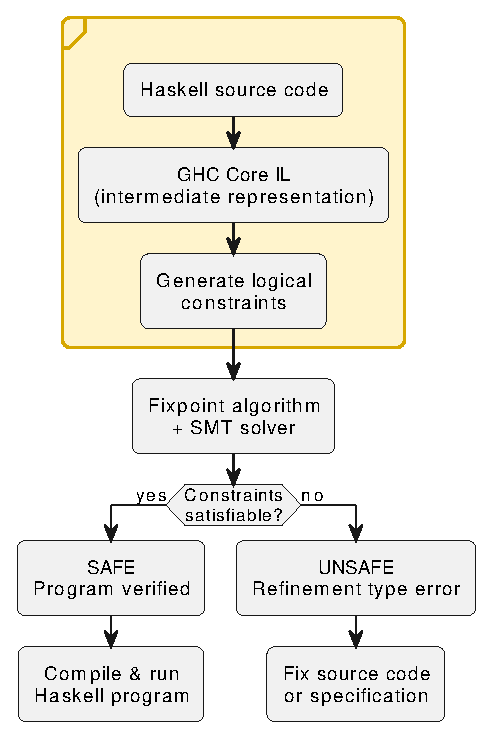
\includegraphics[
				width=\textwidth,
				height=0.9\textheight,
				keepaspectratio
			]{assets/lh-p1.pdf}
		\end{column}
	\end{columns}
\end{frame}

\begin{frame}{LiquidHaskell Architecture}
	\begin{columns}[T]
		\begin{column}{0.6\textwidth}
			\small

			\textbf{Solution}
			\begin{itemize}
				\item A fixpoint algorithm processes the constraints
				\item Any \emph{SMT-LIB2} compatible solver checks whether the constraints can be satisfied (eg.: \emph{Z3}, \emph{CVC4}, \dots)
			\end{itemize}

			\vspace{0.5em}

			\textbf{Result}
			\begin{itemize}
				\item \textbf{SAFE} or \textbf{UNSAFE}: based on the verification of the refinement properties
				\item Errors are mapped back to their source-code locations
			\end{itemize}
		\end{column}

		\begin{column}{0.4\textwidth}
			\centering
			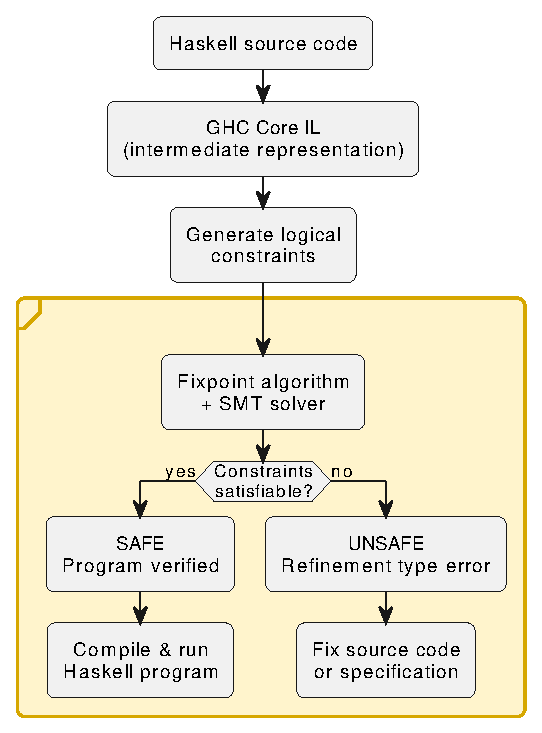
\includegraphics[
				width=\textwidth,
				height=0.9\textheight,
				keepaspectratio
			]{assets/lh-p2.pdf}
		\end{column}
	\end{columns}
\end{frame}

\begin{frame}[fragile]{LiquidHaskell}
	LiquidHaskell is an \textbf{optional} type checker for Haskell. Refinement types are written inside \textbf{comments}, so they are optional and normal Haskell compilers can ignore them:

	\begin{lstlisting}[language=Haskell]
{-@ ... @-}
\end{lstlisting}

	\begin{exampleblock}{Execution}
		\vspace{0.1em}
		LiquidHaskell performs static verification before the Haskell program is executed. It does not become part of the executable or perform any checks during runtime.
	\end{exampleblock}
\end{frame}

\begin{frame}[fragile]{LiquidHaskell Basics}
	\medskip
	\begin{lstlisting}[language=Haskell]
{-@ type Natural = {v:Int | v >= 0} @-}
{-@ type Pos = {v:Int | v > 0} @-}

{-@ increment :: Natural -> Pos @-}
increment :: Int -> Int
increment x = x + 1

good1 = increment 0
good2 = increment 4

-- verification will fail here stating: Type Mismatch
(*@\codeerror{bad = increment (-1)}@*)
\end{lstlisting}

\end{frame}

\begin{frame}[fragile]{LiquidHaskell Basics}
	\medskip
	\begin{lstlisting}[language=Haskell]
{-@ type Natural = {v:Int | v >= 0} @-}
{-@ type Pos = {v:Int | v > 0} @-}

{-@ divide :: n:Natural -> d:Pos -> {v:Natural | v <= n} @-}
divide :: Int -> Int -> Int
divide x y = x `div` y

good = divide 5 2

-- With LH -> Type Mismatch before executing the code
-- Without LH -> runtime error: divide by zero
(*@\codeerror{bad = divide 5 0}@*)
\end{lstlisting}

\end{frame}

\begin{frame}[fragile]{LiquidHaskell Parameterized Types}
	\textbf{Type parameters} are written as lowercase and \textbf{value parameters} are written as uppercase.

	\begin{itemize}
		\item \textbf{Type parameter:} \emph{Int}, \emph{Bool}, \emph{[Int]}
		\item \textbf{Value parameter:} \emph{0}, \emph{10}, \emph{100}
	\end{itemize}

	\begin{lstlisting}[language=Haskell]
{-@ type NonEmpty a = {v:[a] | len v > 0} @-}

{-@ numbers :: NonEmpty Int @-}
numbers :: [Int]
(*@\codeerror{numbers = []}@*)

{-@ letters :: NonEmpty Char @-}
letters :: [Char]
letters = ['a', 'b', 'c']
\end{lstlisting}
\end{frame}

\begin{frame}[fragile]{LiquidHaskell Parameterized Types}
	\medskip
	\begin{lstlisting}[language=Haskell]
{-@ type Rng Low High = {v:Int | v >= Low && v <= High} @-}

{-@ grade :: Rng 0 100 -> Int @-}
grade :: Int -> Int
grade score
    | score >= 90 = 5
    | score >= 75 = 4
    | score >= 60 = 3
    | score >= 50 = 2
    | otherwise   = 1

good = grade 85
(*@\codeerror{bad  = grade 120}@*)
\end{lstlisting}
\end{frame}

\begin{frame}[fragile]{LiquidHaskell Parameterized Types}
	\medskip
	\begin{lstlisting}[language=Haskell]
-- a: element type, N list length
{-@ type ListN a N = {v:[a] | len v == N} @-}

{-@ numbers :: ListN Int 3 @-}
numbers :: [Int]
numbers = [1, 2, 3]

{-@ letters :: ListN Char 2 @-}
letters :: [Char]
letters = ['a', 'b']

{-@ invalid :: ListN Bool 3 @-}
invalid :: [Bool]
(*@\codeerror{invalid = [True, False]}@*)
    \end{lstlisting}
\end{frame}

\begin{frame}[fragile]{LiquidHaskell Type Aliases}
	\textbf{Type Aliases:} used for reusability and readability.
	\begin{lstlisting}[language=Haskell]
-- with type alias
{-@ predicate Between Low High V = V >= Low && V <= High @-}
{-@ type Rng Low High = {v:Int | Between Low High v} @-}

-- we can use the predicate inline as well
{-@ grade :: Rng 0 100 -> {v:Int | Between 1 2 v} @-}
grade :: Int -> Int
grade score
    | score >= 50 = 2
    | otherwise   = 1

good = grade 85
(*@\codeerror{bad  = grade 120}@*)
\end{lstlisting}
\end{frame}

\section{Contracts and Verification}

\begin{frame}[fragile]{LiquidHaskell Function Contracts}
	\begin{itemize}
		\item \textbf{Precondition:} Constraint on the function's inputs.
		\item \textbf{Postcondition:} Constraint on the function's output.
		\item \textbf{Dependent types:} Output constraints can refer to input values.
	\end{itemize}

	\begin{lstlisting}[language=Haskell]
{-@ type Rng Low High = {v:Int | v >= Low && v <= High} @-}

{-@ range :: lo:Int
          -> hi:{Int | hi >= lo}
          -> [Rng lo hi] @-}
range :: Int -> Int -> [Int]
(*@\codeerror{range lo hi = [lo..hi]}@*)

-- [1..5] -> [1, 2, 3, 4, 5]
-- [5..1] -> []
\end{lstlisting}
\end{frame}

\begin{frame}[fragile]{LiquidHaskell Verification: Contracts}
	\medskip
	\begin{lstlisting}[language=Haskell]
{-@ type Rng Low High = {v:Int | v >= Low && v <= High} @-}

{-@ range :: lo:Int
          -> hi:{Int | lo <= hi}
          -> [Rng lo hi] @-}
range :: Int -> Int -> [Int]
(*@\codeerror{range lo hi = [lo..hi]}@*)

good = range 1 5
(*@\codeerror{bad  = range 5 1}@*)
    \end{lstlisting}

	\begin{itemize}
		\item \textbf{SAFE:} range 1 5 satisfies
		      the precondition \(1 \le 5\).
		\item \textbf{UNSAFE:} range 5 1 violates
		      the precondition \(5 \nleq 1\).
	\end{itemize}
\end{frame}

\begin{frame}[fragile]{LiquidHaskell Verification: Limitations}
	\begin{itemize}
		\item Haskell's \texttt{[lo..hi]} is alias for \texttt{enumFromTo lo hi}.
		\item LiquidHaskell relies on refinement specifications to reason about library functions.
		\item Without a sufficiently precise specification for \texttt{enumFromTo}, it cannot prove that every element satisfies \texttt{Rng lo hi}.
	\end{itemize}

	\medskip

	\begin{lstlisting}[language=Haskell]
-- Cannot verify the postcondition
(*@\codeerror{range lo hi = [lo..hi]}@*)
\end{lstlisting}
	\begin{alertblock}{Important}
		\vspace{0.1em}
		\textbf{UNSAFE} does not necessarily mean the code is wrong. It can mean LiquidHaskell cannot prove its correctness.
	\end{alertblock}
\end{frame}

\begin{frame}[fragile]{LiquidHaskell Verification: Recursive Range}
	\begin{lstlisting}[language=Haskell]
{-@ range :: lo:Int
          -> hi:{Int | lo <= hi}
          -> [Rng lo hi] @-}
range :: Int -> Int -> [Int]
range lo hi
  | lo <= hi = lo : range (*@\codeerror{(lo + 1) hi}@*)
  | otherwise = []
\end{lstlisting}

	\begin{itemize}
		\item At \texttt{lo == hi}, the recursive call is \texttt{range (hi + 1) hi}.
		\item Its precondition requires \(hi + 1 \le hi\), which is false.
	\end{itemize}
\end{frame}

\begin{frame}[fragile]{LiquidHaskell Verification: Fixing the Boundary}
	\begin{lstlisting}[language=Haskell]
{-@ range :: lo:Int
          -> hi:{Int | lo <= hi}
          -> [Rng lo hi] @-}
range :: Int -> Int -> [Int]
range lo hi
  | lo < hi   = lo : range (*@\codeerror{(lo + 1)}@*) hi
  | otherwise = [lo]
\end{lstlisting}

	\begin{itemize}
		\item When \texttt{lo < hi}, integer arithmetic gives \(lo + 1 \le hi\).
		\item Otherwise, the precondition implies \texttt{lo == hi}; return the endpoint.
		\item Every returned element satisfies \(lo \le v \le hi\).
		\item By default, LiquidHaskell tries to prove termination using a \textbf{decreasing argument}, but here \texttt{lo} increases instead.
	\end{itemize}
\end{frame}

\begin{frame}{LiquidHaskell Termination}
	Haskell only evaluates expressions when their results are needed (\emph{non-strict evaluation}).

	\begin{itemize}
		\item Some functions may run forever without producing a result.
		\item \textbf{LiquidHaskell:} Must ensure that functions terminate to safely verify certain properties.
		\item By default, LiquidHaskell proves termination of each recursive function.
	\end{itemize}

	\begin{exampleblock}{Termination metric}
		\vspace{0.1em}
		A termination metric is a value that:
		\begin{itemize}
			\item Gets smaller with \textbf{every} recursive call.
			\item Cannot decrease forever (e.g., a non-negative integer).
		\end{itemize}
	\end{exampleblock}
\end{frame}

\begin{frame}[fragile]{LiquidHaskell Termination: Factorial}
	A simple termination metric is a \textbf{non-negative integer}.

	\begin{lstlisting}[language=Haskell]
{-@ fac :: n:Nat -> Nat / [n] @-}
fac :: Int -> Int
fac 0 = 1
fac n = n * fac (n - 1)
\end{lstlisting}

	\begin{itemize}
		\item \texttt{Nat}: integers greater than or equal to zero.
		\item \texttt{/ [n]}: use the argument \texttt{n} as the termination metric.
		\item The base case returns immediately.
		\item The recursive case decreases \texttt{n} by 1 each call.
	\end{itemize}
\end{frame}

\begin{frame}{LiquidHaskell Termination: Proof Obligations}
	Refinement checking establishes the facts needed for \texttt{fac}:

	\begin{itemize}
		\item The input contract gives \(n \ge 0\).
		\item In the recursive branch, \(n \ne 0\), so \(n > 0\).
		\item The next argument remains non-negative: \(n - 1 \ge 0\).
		\item The metric strictly decreases: \(n - 1 < n\).
	\end{itemize}

	\begin{exampleblock}{Why this proves termination}
		\vspace{0.1em}
		A strictly decreasing sequence of non-negative integers cannot continue forever. At zero, the base case stops recursion.
	\end{exampleblock}
\end{frame}

\begin{frame}[fragile]{LiquidHaskell Verification: Proving Termination}
	\medskip
	\begin{lstlisting}[language=Haskell]
{-@ range :: lo:Int
          -> hi:{Int | lo <= hi}
          -> [Rng lo hi] / [hi - lo] @-}
range :: Int -> Int -> [Int]
range lo hi
  | lo < hi   = lo : range (lo + 1) hi
  | otherwise = [lo]
\end{lstlisting}

	\begin{itemize}
		\item \texttt{/ [hi - lo]} supplies an explicit \textbf{termination metric}.
		\item The precondition ensures \(hi - lo \ge 0\).
		\item Each recursive call strictly decreases the metric:
		      \[hi - (lo + 1) = (hi - lo) - 1.\]
		\item At \texttt{lo == hi}, the metric is zero and recursion stops.
	\end{itemize}
\end{frame}

\section{Refining Data and Interfaces}

\begin{frame}[fragile]{LiquidHaskell Measures}
	So far, the specifications have been limited to comparisons and arithmetic operations on \textbf{primitive} values. \textbf{Measures} describe \textbf{inductive properties} of algebraic data types.

	\begin{lstlisting}[language=Haskell]
{-@ measure myLen @-}
myLen :: [a] -> Int
myLen []     = 0
myLen (x:xs) = 1 + myLen xs
\end{lstlisting}

	\begin{itemize}
		\item One equation for each data constructor: \texttt{[]} and \texttt{(:)}.
		\item Each right-hand side must belong to the restricted refinement logic.
		\item \texttt{measure myLen} makes this Haskell function available in refinements; it must obey the measure restrictions.
	\end{itemize}
\end{frame}

\begin{frame}[fragile]{LiquidHaskell Measures: Minimum Length}
	\begin{lstlisting}[language=Haskell]
{-@ type MinLength a N = {v:[a] | myLen v >= N} @-}

{-@ good :: MinLength Int 3 @-}
good :: [Int]
good = [1, 2, 3, 4]

{-@ bad :: MinLength Int 3 @-}
bad :: [Int]
(*@\codeerror{bad = [1, 2]}@*)
\end{lstlisting}

	\begin{itemize}
		\item \texttt{a} is the element type; \texttt{N} is the minimum length.
		\item \textbf{SAFE:} \texttt{good} has length 4, and \(4 \ge 3\).
		\item \textbf{UNSAFE:} \texttt{bad} has length 2, and \(2 < 3\).
	\end{itemize}
\end{frame}

\begin{frame}[fragile]{LiquidHaskell Measures: Constructor Refinements}
	Each list constructor gives LiquidHaskell a \textbf{length fact}:

	\begin{lstlisting}[language=Haskell]
[]  :: {v:[a] | myLen v == 0}

(:) :: x:a -> xs:[a]
    -> {v:[a] | myLen v == 1 + myLen xs}
\end{lstlisting}

	\begin{itemize}
		\item \texttt{[]}: the length is zero.
		\item \texttt{x:xs}: the length is one more than \texttt{xs}.
		\item These facts are available when building or pattern matching on lists.
	\end{itemize}
\end{frame}

\begin{frame}[fragile]{LiquidHaskell Measures: Using a Constructor Fact}
	Adding an element increases the minimum length.

	\begin{lstlisting}[language=Haskell]
{-@ prepend :: a -> MinLength a 2 -> MinLength a 3 @-}
prepend :: a -> [a] -> [a]
prepend x xs = x : xs

good = prepend 1 [2, 3]
(*@\codeerror{bad = prepend 1 [2]}@*)
\end{lstlisting}

	\begin{itemize}
		\item Input contract: \(\mathit{myLen}\;xs \ge 2\).
		\item Constructor fact: \(\mathit{myLen}\;(x:xs) = 1 + \mathit{myLen}\;xs \ge 3\).
	\end{itemize}
\end{frame}

\begin{frame}[fragile]{LiquidHaskell Measures: Function Contracts}
	Measures relate the \textbf{structure of inputs and outputs}.

	\begin{lstlisting}[language=Haskell]
-- Appending adds the lengths
{-@ append :: xs:[a] -> ys:[a]
           -> {v:[a] | myLen v == myLen xs + myLen ys} @-}

-- Mapping preserves the length
{-@ map :: (a -> b) -> xs:[a]
        -> {v:[b] | myLen v == myLen xs} @-}

-- Filtering cannot increase the length
{-@ filter :: (a -> Bool) -> xs:[a]
           -> {v:[a] | myLen v <= myLen xs} @-}
\end{lstlisting}

\end{frame}

\begin{frame}[fragile]{LiquidHaskell Refined Data Types}
	Every value of a data type may need to satisfy an \textbf{invariant}.

	\begin{lstlisting}[language=Haskell]
data CSV a = CSV { cols :: [String], rows :: [[a]] }
\end{lstlisting}

	\begin{itemize}
		\item \texttt{cols}: the column names in the header.
		\item \texttt{rows}: the table's rows, containing values of type \texttt{a}.
		\item Haskell allows rows of different lengths.
	\end{itemize}

	\begin{exampleblock}{CSV invariant}
		\vspace{0.1em}
		Every row must have exactly as many entries as the header has column names.
	\end{exampleblock}
\end{frame}

\begin{frame}[fragile]{LiquidHaskell Refined Data Types: Definition}
	A field's refinement can refer to an \textbf{earlier field}.

	\begin{lstlisting}[language=Haskell]
{-@ type ListL a X = {v:[a] | len v == len X} @-}

{-@ data CSV a = CSV { cols :: [String]
                     , rows :: [ListL a cols] } @-}
\end{lstlisting}

	\begin{itemize}
		\item \texttt{ListL a X}: a list with the same length as \texttt{X}.
		\item \texttt{rows}: a list of rows, each matching the length of \texttt{cols}.
		\item \texttt{len} is LiquidHaskell's built-in list length measure.
	\end{itemize}
\end{frame}

\begin{frame}[fragile]{LiquidHaskell Refined Data Types: Verification}
	\medskip
	\begin{lstlisting}[language=Haskell]
good = CSV ["Month", "Days"]
              [ ["Jan", "31"]
              , ["Feb", "28"]
              , ["Mar", "31"] ]

bad =  CSV ["Month", "Days"]
             [ ["Jan", "31"]
             , ["Feb", "28"]
             , (*@\codeerror{["Mar"]}@*) ]
\end{lstlisting}

\end{frame}

\begin{frame}[fragile]{LiquidHaskell Refined Data Types: Global Invariants}
	Like measures, refined data definitions strengthen \textbf{constructor types}.

	\begin{lstlisting}[language=Haskell]
-- Refined constructor type
CSV :: cols:[String] -> rows:[ListL a cols] -> CSV a
\end{lstlisting}

	\begin{itemize}
		\item Construction checks every row against the header length.
		\item Pattern matching makes this relationship available to the checker.
		\item No extra annotation is needed on individual CSV values.
	\end{itemize}

	\textbf{Global guarantee:} LiquidHaskell rejects CSV-typed expressions that violate this invariant.
\end{frame}

\begin{frame}[fragile]{LiquidHaskell Refined Type Classes}
	A \textbf{type class} defines a shared interface for different types.

	\begin{lstlisting}[language=Haskell]
class Reward a where
  reward :: a -> Int -> Int
\end{lstlisting}

	\begin{itemize}
		\item \texttt{a}: the type that determines the reward policy.
		\item \texttt{reward}: takes a policy value and the current points.
		\item Each instance provides its own implementation.
	\end{itemize}

	\textbf{Shared rule:} points must be non-negative and cannot decrease.
\end{frame}

\begin{frame}[fragile]{LiquidHaskell Refined Type Classes: Contract}
	Refinements specify a \textbf{shared contract} for the class method.

	\begin{lstlisting}[language=Haskell]
{-@ class Reward a where
      reward :: a -> points:{Int | points >= 0}
             -> {v:Int | v >= points}
@-}
\end{lstlisting}

	\begin{itemize}
		\item \textbf{Precondition:} input points must be non-negative.
		\item \textbf{Postcondition:} the result cannot be smaller than the input.
		\item Every instance must satisfy the \textbf{same contract}.
	\end{itemize}
\end{frame}

\begin{frame}[fragile]{LiquidHaskell Refined Type Classes: Bool Instance}
	A Boolean flag decides whether to add a bonus.

	\begin{lstlisting}[language=Haskell]
instance Reward Bool where
  reward bonus points
    | bonus     = points + 10
    | otherwise = points
\end{lstlisting}

	\begin{itemize}
		\item \texttt{True}: add 10 points.
		\item \texttt{False}: keep the original points.
		\item Both branches satisfy \(v \ge points\).
	\end{itemize}

	LiquidHaskell checks the instance against the class contract.
\end{frame}

\begin{frame}[fragile]{LiquidHaskell Refined Type Classes: Verification}
	\begin{lstlisting}[language=Haskell]
good :: Int
good = reward True 20

bad :: Int
(*@\codeerror{bad = reward True (-1)}@*)
\end{lstlisting}

	\begin{itemize}
		\item \textbf{SAFE:} \texttt{good} passes non-negative points and returns 30.
		\item \textbf{UNSAFE:} \texttt{bad} violates the precondition \(points \ge 0\).
	\end{itemize}
\end{frame}

\begin{frame}[fragile]{LiquidHaskell Refined Type Classes: Invalid Instance}
	What if we replace the bonus with a deduction?

	\begin{lstlisting}[language=Haskell]
-- alternative implementation:
instance Reward Bool where
  reward bonus points
    | bonus     = (*@\codeerror{points - 10}@*)
    | otherwise = points
\end{lstlisting}

	\begin{itemize}
		\item The first branch violates \(v \ge points\).
		\item Callers must meet the precondition.
		\item Instances must prove the postcondition.
	\end{itemize}
\end{frame}

\section{Totality and Advanced Termination}

\begin{frame}[fragile]{LiquidHaskell Totality: Missing Patterns}
	A function can pass Haskell's type checker but still fail on some inputs.

	\begin{lstlisting}[language=Haskell]
head :: [a] -> a
head (x:_) = x

good = head [1, 2, 3]
(*@\codeerror{bad = head []}@*)
\end{lstlisting}

	\begin{itemize}
		\item The definition only handles non-empty lists.
		\item An empty list causes a \textbf{pattern-match exception}.
		\item Totality checking must prove that this failure cannot happen.
	\end{itemize}
\end{frame}

\begin{frame}[fragile]{LiquidHaskell Totality: Core Translation}
	GHC makes the missing case explicit in Core:

	\begin{lstlisting}[language=Haskell]
head d = case d of
  x:xs -> x
  []   -> patError "head"
\end{lstlisting}

	\begin{itemize}
		\item Both list constructors now have a branch.
		\item \texttt{patError} throws an exception describing the failed match.
		\item To rule out this exception, prove that the error branch is \textbf{unreachable}.
	\end{itemize}
\end{frame}

\begin{frame}[fragile]{LiquidHaskell Totality: Making Head Safe}
	Restrict the input to \textbf{non-empty lists}.

	\begin{lstlisting}[language=Haskell]
{-@ type NonEmpty a = {v:[a] | len v > 0} @-}
{-@ head :: NonEmpty a -> a @-}
head :: [a] -> a
head (x:_) = x
\end{lstlisting}

	\begin{itemize}
		\item The input contract gives \(\mathit{len}\;v > 0\).
		\item The empty branch gives \(\mathit{len}\;v = 0\): a contradiction.
		\item The error call is unreachable.
	\end{itemize}
\end{frame}

\begin{frame}{LiquidHaskell Termination: Processing Batches}
	Consider a simplified \textbf{batch worker} that counts completed jobs.

	\begin{itemize}
		\item \texttt{b}: batches remaining, including the current batch.
		\item \texttt{j}: jobs remaining in the current batch.
		\item Completing a job decreases \texttt{j}, while \texttt{b} stays unchanged.
		\item Moving to the next batch decreases \texttt{b} and resets \texttt{j} to 3.
	\end{itemize}

	\begin{exampleblock}{Two batches of three jobs}
		\vspace{0.1em}
		\((2,3) \to (2,2) \to (2,1) \to (2,0) \to (1,3) \to \cdots \to (1,0)\).

		\medskip
		Neither argument strictly decreases at every call. We supply a \textbf{custom termination metric}: the pair \texttt{[b, j]}.
	\end{exampleblock}
\end{frame}

\begin{frame}[fragile]{LiquidHaskell Termination: Lexicographic Ordering}
	Compare the \textbf{batch count first}, then the job count.

	\begin{lstlisting}[language=Haskell]
{-@ jobs :: b:Nat -> j:Nat -> Nat / [b, j] @-}
jobs :: Int -> Int -> Int
jobs b j
  | b == 0    = 0
  | j > 0     = 1 + jobs b (j - 1)
  | b == 1    = 0
  | otherwise = jobs (b - 1) 3
-- jobs 2 3 == 6
\end{lstlisting}
\end{frame}

\begin{frame}{LiquidHaskell Termination: Why the Pair Decreases}
	\texttt{/ [b, j]} uses \textbf{lexicographic ordering}: compare \texttt{b} first, and compare \texttt{j} only when \texttt{b} is unchanged.

	\begin{itemize}
		\item \texttt{jobs b (j - 1)}: the first component stays equal, the second decreases.
		\item \texttt{jobs (b - 1) 3}: the first component decreases.
		\item Both components remain non-negative.
		\item At \texttt{b == 0}, or when the last batch is empty (\texttt{b == 1} and \texttt{j == 0}), recursion stops.
	\end{itemize}
\end{frame}

\section{Memory Safety}

\begin{frame}{LiquidHaskell Memory Safety}
	Haskell's high-level libraries can use \textbf{unsafe memory operations} internally for speed.

	\begin{itemize}
		\item \textbf{ByteString:} stores bytes and uses pointer arithmetic.
		\item Refinements track buffer sizes and valid positions.
	\end{itemize}

	\begin{exampleblock}{Main idea}
		\vspace{0.1em}
		Before reading or writing memory, prove that there is enough space.
	\end{exampleblock}
\end{frame}

\begin{frame}[fragile]{LiquidHaskell ByteString: Staying Inside the Buffer}
	A ByteString is a \textbf{slice}: a pointer, a starting offset, and a length.

	\begin{lstlisting}[language=Haskell]
measure fplen :: ForeignPtr a -> Int
data ByteString = PS
 { pay :: ForeignPtr Word8
 , off :: {v:Nat | v       <= (fplen pay)}
 , len :: {v:Nat | off + v <= (fplen pay)} }
\end{lstlisting}

	\begin{itemize}
		\item \texttt{fplen pay}: the buffer size in bytes.
		\item \texttt{off + len} cannot exceed that size.
	\end{itemize}

	\textbf{Paper notation:} refinements are shown directly, without comment wrappers.
\end{frame}

\begin{frame}[fragile]{LiquidHaskell ByteString: Pointer Contracts}
	A pointer with room for \textbf{at least N bytes}:

	\begin{lstlisting}[language=Haskell]
type PtrN a N = {v:Ptr a | N <= (plen v)}
\end{lstlisting}

	\begin{itemize}
		\item \texttt{plen v}: the available buffer size.
		\item Copying N bytes requires that much space in both buffers.
		\item LiquidHaskell checks these requirements at the call site.
	\end{itemize}

	\begin{alertblock}{Trusted boundary}
		\vspace{0.1em}
		Contracts for external C functions are assumed, their C code is not verified.
	\end{alertblock}

	These contracts ensure that copying stays inside both buffers.
\end{frame}

\section{Functional Correctness Invariants}

\begin{frame}[fragile]{LiquidHaskell Functional Correctness}
	Beyond avoiding errors, refinements can express \textbf{application-specific correctness rules}.

	\medskip
	The paper's example: \textbf{red-black trees}, a balanced binary search tree structure.

	\begin{lstlisting}[language=Haskell]
data Col    = R | B
data Tree a = Leaf
            | Node Col a (Tree a) (Tree a)
\end{lstlisting}

	\begin{itemize}
		\item \texttt{Col}: the color; \texttt{a}: the key; followed by the left and right subtrees.
	\end{itemize}
\end{frame}

\begin{frame}{LiquidHaskell Red-Black Trees: Three Invariants}
	A tree is only a valid Red-Black tree if:

	\begin{itemize}
		\item \textbf{Order:} all keys in the left subtree are smaller than the node's keyand all keys in the right subtree are larger.
		\item \textbf{Color:} a red node has only black children. Empty leaves count as black.
		\item \textbf{Height:} from any node, every path to a leaf contains the same number of black nodes.
	\end{itemize}

	\begin{exampleblock}{Main idea}
		\vspace{0.1em}
		Describe these properties separately, then combine them without changing the underlying tree structure.
	\end{exampleblock}
\end{frame}

\begin{frame}{LiquidHaskell Red-Black Trees: Valid and Invalid}
	\tikzset{
		rbNode/.style={circle, text=white, minimum size=0.65cm, inner sep=0pt},
		rbBlack/.style={rbNode, fill=themeText},
		rbRed/.style={rbNode, fill=themeAlert},
		rbLeaf/.style={rectangle, fill=themeText, minimum size=0.25cm, inner sep=0pt}
	}

	\begin{columns}[T]
		\begin{column}{0.5\textwidth}
			\centering
			\textcolor{themeExample}{\textbf{Valid}}

			\medskip
			\begin{tikzpicture}[
					level 1/.style={level distance=0.95cm, sibling distance=1.8cm},
					level 2/.style={level distance=0.65cm, sibling distance=0.7cm},
					edge from parent/.style={draw=themeText}
				]
				\node[rbBlack] {10}
				child {node[rbRed] {5}
						child {node[rbLeaf] {}}
						child {node[rbLeaf] {}}}
				child {node[rbRed] {15}
						child {node[rbLeaf] {}}
						child {node[rbLeaf] {}}};
			\end{tikzpicture}

			\medskip
			\(5 < 10 < 15\).

			Color and height are valid too.
		\end{column}

		\begin{column}{0.5\textwidth}
			\centering
			\textcolor{themeAlert}{\textbf{Invalid}}

			\medskip
			\begin{tikzpicture}[
					level 1/.style={level distance=0.95cm, sibling distance=1.8cm},
					level 2/.style={level distance=0.65cm, sibling distance=0.7cm},
					edge from parent/.style={draw=themeText}
				]
				\node[rbBlack] {10}
				child {node[rbRed] {12}
						child {node[rbLeaf] {}}
						child {node[rbLeaf] {}}}
				child {node[rbRed] {15}
						child {node[rbLeaf] {}}
						child {node[rbLeaf] {}}};
			\end{tikzpicture}

			\medskip
			\textbf{Order fails:} \(12 > 10\).
		\end{column}
	\end{columns}

	\vspace{2em}
	\centering
	\emph{Black squares represent empty leaves.}
\end{frame}

\begin{frame}[fragile]{LiquidHaskell Red-Black Trees: Checking Color}
	\begin{lstlisting}[language=Haskell]
measure isB :: Tree a -> Prop
isB (Node c x l r) = c == B
isB (Leaf) = true

measure isRB :: Tree a -> Prop
isRB (Leaf) = true
isRB (Node c x l r) = isRB l && isRB r &&
                    c == R => (isB l && isB r)
\end{lstlisting}

	\begin{itemize}
		\item \texttt{isB}: the root is black; empty leaves count as black.
		\item \texttt{isRB}: red nodes have black children, recursively.
	\end{itemize}
\end{frame}

\begin{frame}[fragile]{LiquidHaskell Red-Black Trees: Checking Height}
	\begin{lstlisting}[language=Haskell]
measure bh :: Tree a -> Int
bh (Leaf) = 0
bh (Node c x l r) = bh l + if c == R then 0 else 1

measure isBal :: Tree a -> Prop
isBal (Leaf) = true
isBal (Node c x l r) = bh l == bh r && isBal l && isBal r
\end{lstlisting}

	\begin{itemize}
		\item \texttt{bh}: count black nodes along the leftmost path.
		\item \texttt{isBal}: require equal black heights, recursively.
	\end{itemize}
\end{frame}

\begin{frame}[fragile]{LiquidHaskell Red-Black Trees: Checking Order}
	\begin{lstlisting}[language=Haskell]
data Tree a <l :: a -> a -> Prop,
             r :: a -> a -> Prop>
  = Leaf
  | Node { c   :: Col
         , key :: a
         , lt  :: Tree <l, r> a <l key>
         , rt  :: Tree <l, r> a <r key> }
type OTree a
  = Tree <{\k v -> v < k},   -- l: left rule
          {\k v -> v > k}> a -- r: right rule
\end{lstlisting}

	\begin{itemize}
		\item \texttt{l} and \texttt{r}: rules relating keys to subtree values.
		\item \texttt{OTree}: left keys \(v < k\); right keys \(v > k\).
	\end{itemize}
\end{frame}

\begin{frame}[fragile]{LiquidHaskell Red-Black Trees: Combining the Rules}
	Combining ordering, color, and black-height balance:

	\begin{lstlisting}[language=Haskell]
type RBT a = {v:OTree a | isRB v && isBal v}
\end{lstlisting}

	\begin{itemize}
		\item \texttt{OTree}: keys follow binary-search ordering.
		\item \texttt{isRB}: red nodes have black children.
		\item \texttt{isBal}: all paths have equal black heights.
	\end{itemize}

	With these invariants and suitable function signatures, LiquidHaskell verifies the library's \textbf{insertion, deletion, and rebalancing} procedures.
\end{frame}

\begin{frame}{LiquidHaskell Stack Sets in XMonad}
	\textbf{xmonad} is a dynamically tiling X11 window manager, written and configured in Haskell.

	\begin{itemize}
		\item The managed windows are organized into a \textbf{hierarchy of types}.
		\item Every level stores windows, together with layout and screen data.
	\end{itemize}

	\begin{exampleblock}{Key invariant}
		\vspace{0.1em}
		Each window appears \textbf{at most once}: it is never duplicated across stacks or workspaces.
	\end{exampleblock}
\end{frame}

\begin{frame}[fragile]{LiquidHaskell XMonad: The Stack Zipper}
	At the lowest level, windows are stored in a \textbf{zipper}:

	\begin{lstlisting}[language=Haskell]
data Stack a = Stack { focus :: a
                     , up    :: [a]
                     , down  :: [a] }
\end{lstlisting}

	\begin{center}
		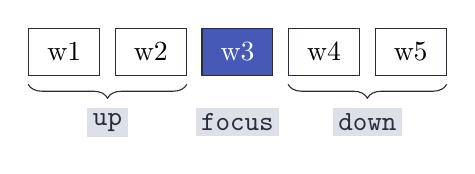
\begin{tikzpicture}[
				win/.style={rectangle, draw=themeText, minimum width=0.9cm, minimum height=0.6cm},
				focused/.style={win, fill=themeAccent, text=white}
			]
			\node[win]     (w1) at (0, 0)   {w1};
			\node[win]     (w2) at (1.1, 0) {w2};
			\node[focused] (w3) at (2.2, 0) {w3};
			\node[win]     (w4) at (3.3, 0) {w4};
			\node[win]     (w5) at (4.4, 0) {w5};
			\draw[decorate, decoration={brace, amplitude=5pt, mirror}, draw=themeText]
			([yshift=-3pt]w1.south west) -- node[below=5pt] {\texttt{up}} ([yshift=-3pt]w2.south east);
			\node[below=8pt] at (w3.south) {\texttt{focus}};
			\draw[decorate, decoration={brace, amplitude=5pt, mirror}, draw=themeText]
			([yshift=-3pt]w4.south west) -- node[below=5pt] {\texttt{down}} ([yshift=-3pt]w5.south east);
		\end{tikzpicture}
	\end{center}

	\begin{itemize}
		\item \texttt{focus}: the current window.
		\item \texttt{up} and \texttt{down}: the windows before and after it.
	\end{itemize}
\end{frame}

\begin{frame}[fragile]{LiquidHaskell XMonad: Type Hierarchy}
	\medskip
	\begin{lstlisting}[language=Haskell]
data Workspace i l a = Workspace
  { tag :: i, layout :: l, stack :: Maybe (Stack a) }

data Screen i l a sid sd = Screen
  { workspace :: Workspace i l a
  , screen :: sid
  , screenDetail :: sd }

data StackSet i l a sid sd = StackSet
  { cur :: Screen i l a sid sd       -- focused screen
  , vis :: [Screen i l a sid sd]     -- other visible screens
  , hid :: [Workspace i l a]         -- hidden workspaces
  , flt :: M.Map a RationalRect }    -- floating windows
\end{lstlisting}
\end{frame}

\begin{frame}[fragile]{LiquidHaskell XMonad: Unique Lists}
	A measure collects the elements of a list into a \textbf{set}:

	\begin{lstlisting}[language=Haskell]
measure elts :: [a] -> Set a
elts ([])   = emp
elts (x:xs) = cup (sng x) (elts xs)

measure isUniq :: [a] -> Prop
isUniq ([])   = true
isUniq (x:xs) = notIn x xs && isUniq xs

predicate notIn X S = not (mem X (elts S))
\end{lstlisting}

	\begin{itemize}
		\item \texttt{emp}, \texttt{sng}, \texttt{cup}: empty set, singleton, union (\(\emptyset\), \(\{x\}\), \(\cup\)).
		\item \texttt{mem}: set membership (\(\in\)).
		\item \texttt{isUniq}: no element occurs in the rest of the list.
	\end{itemize}
\end{frame}

\begin{frame}[fragile]{LiquidHaskell XMonad: Unique Stacks}
	\begin{lstlisting}[language=Haskell]
data Stack a = Stack
  { focus :: a
  , up    :: {v:[a] | Uniq1 v focus}
  , down  :: {v:[a] | Uniq2 v focus up} }

predicate Uniq1 V X   = isUniq V && notIn X V
predicate Uniq2 V X Y = Uniq1 V X && disjoint Y V
predicate disjoint X Y = cap (elts X) (elts Y) = emp
\end{lstlisting}

	\begin{itemize}
		\item \texttt{cap}: set intersection (\(\cap\)); \texttt{disjoint} means no shared elements.
		\item \texttt{up}: a unique list that does not contain \texttt{focus}.
		\item \texttt{down}: the same, and also disjoint from \texttt{up}.
	\end{itemize}
\end{frame}

\begin{frame}[fragile]{LiquidHaskell XMonad: Unique Stack Sets}
	\texttt{elts} and \texttt{isUniq} are lifted to \texttt{Stack}, \texttt{Workspace} and \texttt{Screen}.

	\begin{lstlisting}[language=Haskell]
type UniqStackSet i l a sid sd
  = {v:StackSet i l a sid sd | NoDups v}

predicate NoDups V = disjoint3 (hid V) (cur V) (vis V)
                  && isUniq (vis V) && isUniq (hid V)

predicate disjoint3 X Y Z
  = disjoint X Y && disjoint Y Z && disjoint X Z
\end{lstlisting}

	\begin{itemize}
		\item Record selectors (\texttt{cur}, \texttt{vis}, \texttt{hid}) automatically become measures.
		\item No window is shared between the current, visible and hidden parts.
	\end{itemize}
\end{frame}

\begin{frame}[fragile]{LiquidHaskell XMonad: Strengthening Library Functions}
	xmonad often concatenates \texttt{up s ++ down s}. Proving the result unique needs a stronger type for \texttt{(++)}:

	\begin{lstlisting}[language=Haskell]
-- assumed: two unique, disjoint lists give a unique list
(++) :: xs:{[a] | isUniq xs}
     -> ys:{[a] | isUniq ys && disjoint xs ys}
     -> {v:[a] | isUniq v}

(*@\codeerror{"StackSet" ++ "error"}@*)  -- violates the precondition
\end{lstlisting}

	\begin{itemize}
		\item Not every call concatenates unique, disjoint lists.
		\item LiquidHaskell has no \textbf{intersection types}, so an unrefined \texttt{(++.)} is used for those cases.
	\end{itemize}
\end{frame}

\begin{frame}[fragile]{LiquidHaskell XMonad: Restricting the Domain}
	Given a default value \texttt{x}, a function \texttt{f} and a stack set \texttt{s}, \texttt{modify} applies \texttt{f} to the \texttt{Maybe (Stack a)} values inside \texttt{s}.

	\begin{lstlisting}[language=Haskell]
modify :: Maybe (Stack a)                -- x: default
       -> (Stack a -> Maybe (Stack a))   -- f: update
       -> StackSet i l a s sd            -- s: input
       -> StackSet i l a s sd
\end{lstlisting}

	\begin{itemize}
		\item It should not introduce a \textbf{duplicate window}.
	\end{itemize}
\end{frame}

\begin{frame}[fragile]{LiquidHaskell XMonad: Restricting the Domain}
	The refined type only accepts arguments that preserve uniqueness:

	\begin{lstlisting}[language=Haskell]
modify :: x:{v:Maybe (Stack a) | isNothing v}
       -> (y:Stack a -> Maybe {v:Stack a | SubElts v y})
       -> UniqStackSet i l a s sd
       -> UniqStackSet i l a s sd
\end{lstlisting}

	\begin{itemize}
		\item \texttt{f}: the new stack may only contain windows of \texttt{y}: \(\mathit{elts}\;v \subseteq \mathit{elts}\;y\).
		\item \texttt{x}: its windows could already exist elsewhere in \texttt{s}, so the only safe default is \texttt{Nothing}.
		\item Result: \texttt{s} stays a \texttt{UniqStackSet}.
	\end{itemize}

	\textbf{Precondition:} the default value must be \texttt{Nothing}.
\end{frame}

\begin{frame}{LiquidHaskell XMonad: Summary}
	Verifying the uniqueness invariant required changes to the code and its specifications:

	\begin{itemize}
		\item \textbf{Strengthening library functions:} a stronger type for \texttt{(++)}, plus an unrefined \texttt{(++.)} for other uses.
		\item \textbf{Restricting the domain:} \texttt{modify} only accepts \texttt{Nothing} as its default.
	\end{itemize}

	\begin{exampleblock}{Takeaway}
		\vspace{0.1em}
		Real code sometimes needs \textbf{small rewrites} to verify.
	\end{exampleblock}
\end{frame}

\section{Evaluation}

\begin{frame}{LiquidHaskell Evaluation: Benchmarks}
	\footnotesize
	\centering
	\begin{tabular}{@{}ll@{}}
		\toprule
		\textbf{Library}    & \textbf{Verified properties}                      \\
		\midrule
		GHC.List, Data.List & size properties of list operations                \\
		Data.Set.Splay      & termination, well-ordered splay trees             \\
		Data.Map.Base       & termination, binary-search ordered trees          \\
		HsColour            & totality of all functions                         \\
		XMonad              & window uniqueness, some QuickCheck properties     \\
		ByteString          & termination, memory safety, correctness           \\
		Text                & pointer safety, correctness (\alert{found a bug}) \\
		Vector-Algorithms   & safe vector accessing, indexing and slicing       \\
		\bottomrule
	\end{tabular}
\end{frame}

\begin{frame}{LiquidHaskell Evaluation: Results}
	\centering
	\resizebox{\textwidth}{!}{%
		\begin{tabular}{@{}lrrrrrrr@{}}
			\toprule
			\textbf{Module}   & \textbf{LOC} & \textbf{Mod} & \textbf{Fun} & \textbf{Specs} & \textbf{Annot} & \textbf{Qualif} & \textbf{Time (s)} \\
			\midrule
			GHC.List          & 309          & 1            & 66           & 29 / 38        & 6 / 6          & 0 / 0           & 15                \\
			Data.List         & 504          & 1            & 97           & 15 / 26        & 6 / 6          & 3 / 3           & 11                \\
			Data.Map.Base     & 1396         & 1            & 180          & 125 / 173      & 13 / 13        & 0 / 0           & 174               \\
			Data.Set.Splay    & 149          & 1            & 35           & 27 / 37        & 5 / 5          & 0 / 0           & 27                \\
			HsColour          & 1047         & 16           & 234          & 19 / 40        & 5 / 5          & 1 / 1           & 196               \\
			XMonad.StackSet   & 256          & 1            & 106          & 74 / 213       & 3 / 3          & 4 / 4           & 27                \\
			ByteString        & 3505         & 8            & 569          & 307 / 465      & 55 / 55        & 47 / 124        & 294               \\
			Text              & 3128         & 17           & 493          & 305 / 717      & 52 / 54        & 49 / 97         & 499               \\
			Vector-Algorithms & 1218         & 10           & 99           & 76 / 266       & 9 / 9          & 13 / 13         & 89                \\
			\midrule
			\textbf{Total}    & 11512        & 56           & 1879         & 977 / 1975     & 154 / 156      & 117 / 242       & 1336              \\
			\bottomrule
		\end{tabular}%
	}

	\raggedright
	\footnotesize
	\medskip
	\textbf{Specs, Annot, Qualif:} count / lines of type specifications, other annotations (invariants, termination hints) and qualifiers.
\end{frame}

\begin{frame}{LiquidHaskell Evaluation: What the Numbers Show}
	\begin{itemize}
		\item \textbf{11,512} lines of code in 56 modules, checked with \textbf{1,975} lines of specifications.
		\item Hints (annotations and qualifiers) add only \textbf{3.5\%} of the code size.
	\end{itemize}

	\begin{exampleblock}{Performance}
		\vspace{0.1em}
		The full suite takes about \textbf{22 minutes}, but checking a handful of functions in isolation is fast enough for \textbf{interactive use}.
	\end{exampleblock}
\end{frame}

\begin{frame}{LiquidHaskell Limitations}
	The case studies also showed limitations of LiquidHaskell.

	\begin{itemize}
		\item Ghost parameters
		\item Fixed-width integers and floating-point numbers
		\item Higher-order functions
		\item Functions as data
		\item Lazy binders
		\item Assumes
		\item Error messages
	\end{itemize}

	\begin{exampleblock}{Workaround}
		\vspace{0.1em}
		In most cases, the code could be \textbf{altered slightly} to make verification possible.
	\end{exampleblock}
\end{frame}

\begin{frame}{LiquidHaskell Limitations: Ghost Parameters and Numbers}
	\textbf{Ghost parameters}
	\begin{itemize}
		\item Some values are not needed for the computation, only for the proof.
		\item They must still be passed as extra arguments.
	\end{itemize}

	\medskip
	\textbf{Fixed-width integers and floating-point numbers}
	\begin{itemize}
		\item Numbers are modelled with linear arithmetic and real numbers.
		\item Some precision is lost, e.g.\ bitwise operations can only be approximated.
	\end{itemize}
\end{frame}

\end{document}
